
\begin{center}
\Huge
Funktionstyper 
\end{center}
\section*{Sammensatte funktioner}
\stepcounter{section}
En sammensat funktion er - som navnet hentyder til - funktioner, der er sat sammen. Mere præcist har vi en definition.
\begin{defn}
Har vi to funktioner $f:A \to B$ og $g:B \to C$, så kan vi bestemme  den sammensatte funktion af $f$ og $g$ som
\begin{align*}
g(f(x)).
\end{align*}
Dette skrives også til tider $g(f(x))= g\circ f(x)$. I dette tilfælde kaldes $g$ for den \textit{indre} funktion og $f$ for den \textit{ydre} funktion.
\end{defn}
\begin{figure}[H]
	\centering
	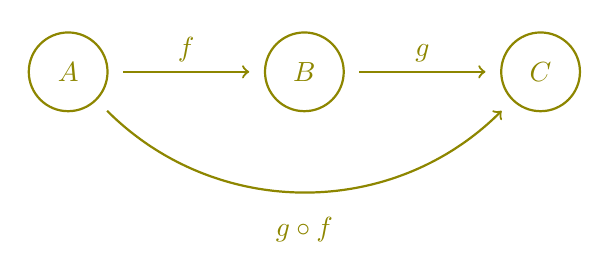
\begin{tikzpicture}
		\draw[color = olive, thick] (0,0) circle (0.5cm);
		\draw[color = olive, thick] (3,0) circle (0.5cm);
		\draw[color = olive, thick] (6,0) circle (0.5cm);
		\node[color = olive] at (0,0) {$A$};
		\node[color = olive] at (3,0) {$B$};
		\node[color = olive] at (6,0) {$C$};
		\draw[-{to[scale = 1.3]}, color = olive, thick] (0.7,0) --(2.3,0) node[midway, anchor = south] {$f$};
		\draw[-{to[scale = 1.3]}, color = olive, thick] (3.7,0) --(5.3,0) node[midway, anchor = south] {$g$};
		\draw[-{to[scale = 1.3]}, color = olive, thick] (0.495,-0.495) to[out = -45, in = 45-180] (5.505,-0.495);
		\node[color = olive] at (3,-2) {$g \circ f$};
	\end{tikzpicture}
\end{figure}
\begin{exa}
Lad $f$ og $g$ være givet ved henholdsvist
\begin{align*}
f(x) = \sqrt{x} \textnormal{ og }g(x) = 3\cdot x.
\end{align*}
Så er den sammensatte funktion $f(g(x))$ bestemt ved
\begin{align*}
f(g(x)) = \sqrt{3\cdot x}.
\end{align*}
Tilsvarende er den sammensatte funktion $g(f(x))$ bestemt ved
\begin{align*}
g(f(x)) = 3\sqrt{x}.
\end{align*}
\end{exa}
\begin{exa}
CO$_2$-koncentrationen i en beholder kan tilnærmes ved $f(x) = 10\cdot x+385$, hvor $f$ er i ppm (parts per million) og $x$ er antallet af en bestemt type bakterier i mio. Antallet af bakterier (i mio.) i beholderen kan i et begrænset tidsinterval beskrives ved $g(t)= 2\cdot 1.07^t$, hvor $t$ beskriver tiden i timer. CO$_2$-koncentrationen som funktion af tid kan derfor beskrives ved
\begin{align*}
f(g(t)) = 10\cdot (2\cdot 1.07^t) + 385 = 20\cdot 1.07^t + 385.
\end{align*}
\section*{Stykvist definerede funktioner}
\stepcounter{section}
En stykvist defineret funktion er en funktion, der er defineret på forskellige måder alt efter hvad $x$ er.
\begin{exa}
Et taxafirma tager følgende pris for taxakørsel: De første to kilometer koster 10kr pr kilometer, de næste 5km koster 7 kr pr kilometer, og resten at afstanden koster taxaen 5kr pr kilometer. Vi kan definere prisen $p(x)$ som en stykvist defineret funktion:
\begin{align*}
p(x)=
\begin{cases}
10\cdot x, \ &0\leq x \leq 2,\\
7\cdot x + 6,\ &2 < x \leq 7,\\
5 \cdot x + 20,\ &7<x,
\end{cases}
\end{align*}
hvor $x$ er antal kilometer kørt og $p(x)$ er prisen i kr. 
\end{exa}
Grafen for $p$ kan ses på Figur \ref{fig:stykvis}.
\begin{figure}[H]
\centering
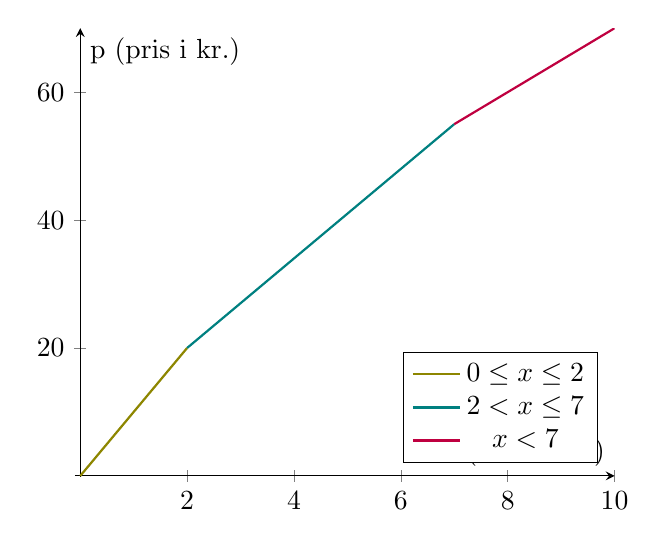
\begin{tikzpicture}
\begin{axis}[axis lines=middle, xmin = -0.1,ymin=-0.1,
legend pos = south east, 
xlabel={x (kørte km.)},
ylabel = {p (pris i kr.)}
]
\addplot[color=olive,samples = 100, thick, domain = 0:2] {10*x};
\addplot[color=teal,samples = 100,thick,domain=2:7] {7*x+6};
\addplot[color=purple,samples = 100,thick,domain=7:10] {5*x+20};
\legend{$0\leq x \leq 2$,$2<x\leq 7$,$x<7$}
\end{axis}
\end{tikzpicture}
\caption{Pris for taxa som funktion af kørte km.}
\label{fig:stykvis}
\end{figure}
\end{exa}
\subsection*{Opgave 1}
En stykvist defineret funktion $f$ er givet ved
\begin{align*}
	f(x) = 
	\begin{cases}
		2x+4, \ &\textnormal{hvis } x < -2,\\
		-4x + 12, \ &\textnormal{hvis } x \geq -2.
	\end{cases}
\end{align*}

\begin{enumerate}[label=\roman*)]
	\item Bestem $f(-2)$.
	\item Bestem $f(-5)$.
	\item Løs ligningen $f(x) = 0$.
\end{enumerate}

\subsection*{Opgave 2}
En stykvist defineret funktion $f$ er givet ved følgende graf. 
\begin{center}
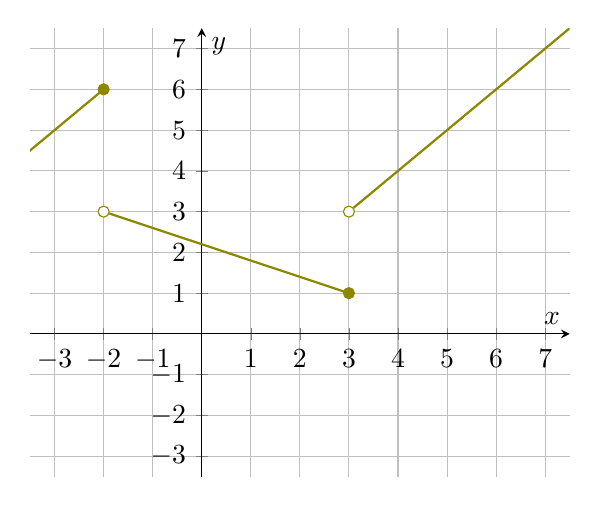
\begin{tikzpicture}
	\begin{axis}
	[axis lines = center, 
	xmin = -3.5, xmax = 7.5,
	ymin = -3.5, ymax = 7.5,
	grid = both,
	xtick = {-3,-2,...,6,7},
	ytick = {-3,-2,...,6,7},
	xlabel = $x$, ylabel = $y$
	]
		\addplot[color = olive, thick, domain = -2:3] {-2/5*x+2.2};
		\addplot[color = olive, thick, domain = 3:10] {x};	
		\addplot[color = olive, thick, domain = -4:-2] {x + 8};	
		\filldraw[color = white](axis cs: -2,3) circle (2pt);
		\filldraw[color = olive](axis cs: 3,1) circle (2pt);
		\draw[color = olive](axis cs: -2,3) circle (2pt);
		\filldraw[color = white](axis cs: 3,3) circle (2pt);
		\draw[color = olive](axis cs: 3,3) circle (2pt);
		\filldraw[color = olive](axis cs: -2,6) circle (2pt);
	\end{axis}
\end{tikzpicture}
\end{center}
\begin{enumerate}[label=\roman*)]
	\item Bestem $f(4)$
	\item Bestem $f(3)$
	\item Løs ligningen $f(x) = 6$
\end{enumerate}

\newpage
 
\subsection*{Opgave 3}
Bestem en forskrift for følgende stykvist definerede funktioner.
\begin{center}
\resizebox{0.45\textwidth}{!}{
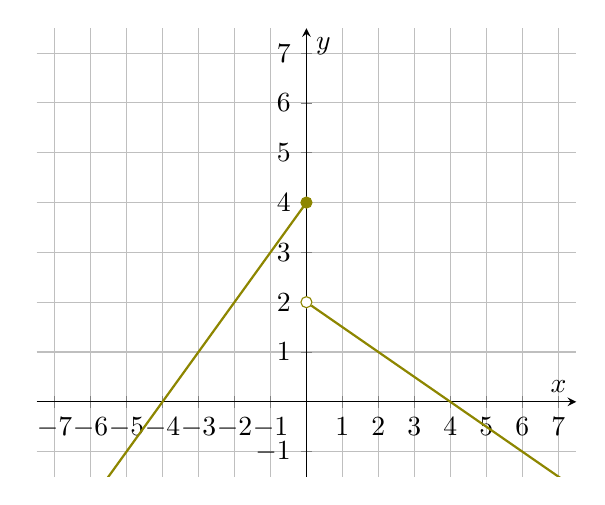
\begin{tikzpicture}
	\begin{axis}
	[axis lines = center, 
	xmin = -7.5, xmax = 7.5,
	ymin = -1.5, ymax = 7.5,
	grid = both,
	xtick = {-7,-6,...,6,7},
	ytick = {-3,-2,...,6,7},
	xlabel = $x$, ylabel = $y$
	]
		\addplot[color = olive, thick, domain = -8:0] {x + 4};
		\addplot[color = olive, thick, domain = 0:8] {-0.5*x + 2};	
		\filldraw[color = olive](axis cs: 0,4) circle (2pt);
		\filldraw[color = white](axis cs: 0, 2 ) circle (2pt);
		\draw[color = olive](axis cs: 0, 2 ) circle (2pt);
	\end{axis}
\end{tikzpicture}
}
\resizebox{0.45\textwidth}{!}{
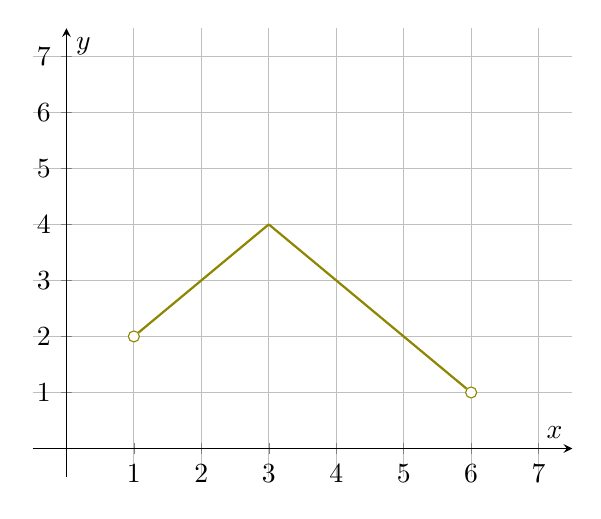
\begin{tikzpicture}
	\begin{axis}
	[axis lines = center, 
	xmin = -0.5, xmax = 7.5,
	ymin = -0.5, ymax = 7.5,
	grid = both,
	xtick = {-3,-2,...,6,7},
	ytick = {-3,-2,...,6,7},
	xlabel = $x$, ylabel = $y$
	]
		\addplot[color = olive, thick, domain = 1:3] {x + 1};
		\addplot[color = olive, thick, domain = 3:6] {-x + 7};	
		\filldraw[color = white](axis cs: 1,2) circle (2pt);
		\filldraw[color = white](axis cs: 6,1) circle (2pt);
		\draw[color = olive](axis cs: 1,2) circle (2pt);
		\draw[color = olive](axis cs: 6,1) circle (2pt);
	\end{axis}
\end{tikzpicture}
}
\resizebox{0.45\textwidth}{!}{
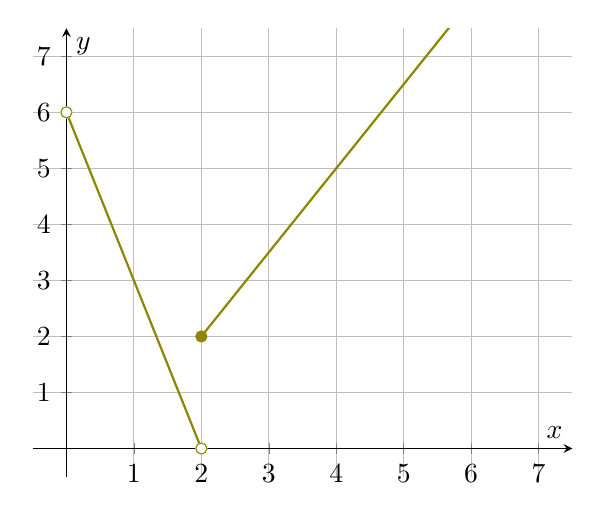
\begin{tikzpicture}
	\begin{axis}
	[axis lines = center, 
	xmin = -0.5, xmax = 7.5,
	ymin = -0.5, ymax = 7.5,
	grid = both,
	xtick = {-3,-2,...,6,7},
	ytick = {-3,-2,...,6,7},
	xlabel = $x$, ylabel = $y$
	]
		\addplot[color = olive, thick, domain = 0:2] {-3*x + 6};
		\addplot[color = olive, thick, domain = 2:6] {1.5*x - 1};	
		\filldraw[color = white](axis cs: 0,6) circle (2pt);
		\filldraw[color = white](axis cs: 2,0) circle (2pt);
		\draw[color = olive](axis cs: 0,6) circle (2pt);
		\draw[color = olive](axis cs: 2,0) circle (2pt);
		\filldraw[color = olive] (axis cs: 2,2) circle (2pt);
	\end{axis}
\end{tikzpicture}
}


\end{center}

\newpage

\subsection*{Opgave 4}
Følgende tre stykvist definerede funktioner er givet
\begin{align*}
	f(x) &=
	\begin{cases}
		x+5, \ &\textnormal{hvis }-3 \leq x < -2,\\
		-0.5x + 4, \ &\textnormal{hvis }-2 \leq x < 2.
	\end{cases}
	\\
	g(x) &=
	\begin{cases}
		-2x-2, \ &\textnormal{hvis }-5 < x \leq 3,\\
		x-11, \ &\textnormal{hvis }3 < x < 5.
	\end{cases}
	\\
	h(x) &=
	\begin{cases}
		x + 5, \ &\textnormal{hvis }-5 < x < -4,\\
		x+ 2, \ &\textnormal{hvis }-4 \leq  x < 0,\\
		-x + 7, \ &\textnormal{hvis }0 \leq x < 2.
	\end{cases}
\end{align*}

\begin{center}
\resizebox{0.45\textwidth}{!}{
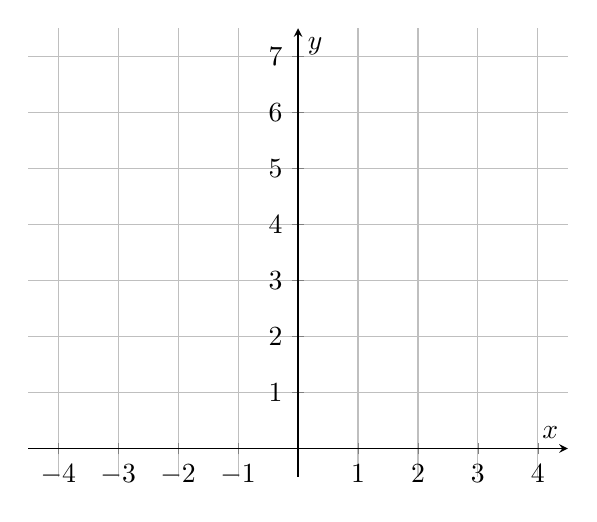
\begin{tikzpicture}
	\begin{axis}
	[axis lines = center, 
	xmin = -4.5, xmax = 4.5,
	ymin = -0.5, ymax = 7.5,
	grid = both,
	xtick = {-4,-3,...,6,7},
	ytick = {-3,-2,...,6,7},
	xlabel = $x$, ylabel = $y$
	]
	\end{axis}
\end{tikzpicture}
}
\resizebox{0.45\textwidth}{!}{
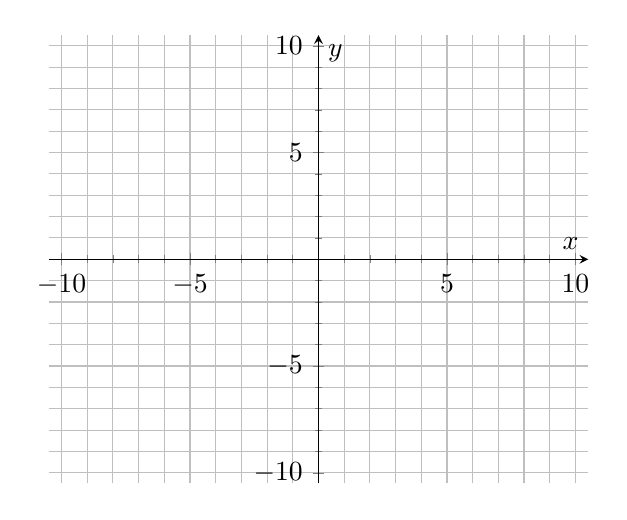
\begin{tikzpicture}
	\begin{axis}
	[axis lines = center, 
	xmin = -10.5, xmax = 10.5,
	ymin = -10.5, ymax = 10.5,
	grid = both,
	xtick = {-10,-5,...,5,10},
	minor tick num = 4,
	ytick = {-10,-5,...,5,10},
	xlabel = $x$, ylabel = $y$
	]
	\end{axis}
\end{tikzpicture}
}
\resizebox{0.45\textwidth}{!}{
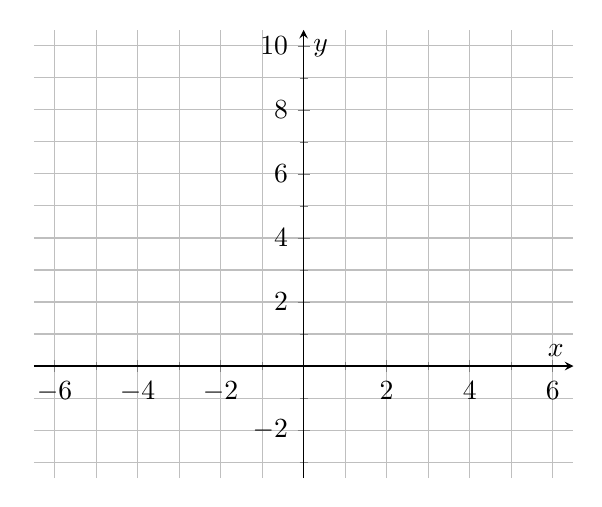
\begin{tikzpicture}
	\begin{axis}
	[axis lines = center, 
	xmin = -6.5, xmax = 6.5,
	ymin = -3.5, ymax = 10.5,
	grid = both,
	xtick = {-10,-8,...,8,10},
	ytick = {-10,-8,...,8,10},
	minor tick num = 1,
	xlabel = $x$, ylabel = $y$
	]
	\end{axis}
\end{tikzpicture}
}
\end{center}


\subsection*{Opgave 5}
For følgende funktioner $f$ og $g$, bestem så den sammensatte funktion $f(g(x))$ og $g(f(g))$.
\begin{align*}
&f(x) = \sqrt{x}\  \textnormal{ og } g(x) = x^2\\
&f(x) = 2x^3\  \textnormal{ og } g(x) = 10x+3\\
&f(x) = \ln(x)\  \textnormal{ og } g(x) = \frac{1}{x}\\
&f(x) = \sqrt[10]{x}\  \textnormal{ og } g(x) = x^{20}
\end{align*}
\subsection*{Opgave 6}
For $f(x) = x^2$ og $g(x)=2x+3$ løs ligningen
\begin{align*}
f(g(x)) = 0.
\end{align*}

\subsection*{Opgave 7}
Bestem for følgende funktion den indre og ydre funktion
\begin{align*}
	&1) \ \sqrt{2x+1}   &&2) \  2^{x^2-7}     \\
	&3) \ \frac{1}{-4x+12}   &&4) \ e^{2x-4}      \\
	&5) \ \ln(2x)   &&6) \  \log_5(7x^2)     \\
	&7) \ (x+10)^3   &&8) \  3^{\log_{10}(2x)+7}       \\
\end{align*}


\subsection*{Opgave 8}
En stykvist defineret funktion $f$ er givet ved
\begin{align*}
	f(x) = 
	\begin{cases}
		x^2, \ &\textnormal{ hvis } x > \geq 0,\\
		-x^2, \ &\textnormal{ hvis } x < 0.
	\end{cases}
\end{align*}
\begin{enumerate}[label=\roman*)]
	\item Bestem $f(3).$
	\item Bestem $f(-4).$
	\item Løs ligningen $f(x) = -64$.
\end{enumerate}

\subsection*{Opgave 9}
Prisen for at rejse $x$ kilometer med taxafirmaet taxA kan beskrives ved funktionen $f$ givet ved
\begin{align*}
	f(x) =
	\begin{cases}
		20x + 50, \ &\textnormal{ hvis } x \leq 8, \\
		16x + 82, \ &\textnormal{ hvis } 8 < x \leq 15, \\
		12x + 142, \ &\textnormal{ hvis } 15 < x.
	\end{cases}
\end{align*}

\begin{enumerate}[label = \roman*)]
	\item Bestem prisen for at køre 10km med taxA.
	\item Afgør, hvor langt man kan køre for 250 kr.
	\item Tegn grafen for $f$ i Maple og verificér dit svar fra i) og ii).
\end{enumerate}

